\section{Resoconto delle attività di verifica\textsubscript{g}}
\subsection{Verifica della qualità dei processi\textsubscript{g}}
In questa sezione vengono riportati i risultati dell'attività di verifica\textsubscript{g} effettuata relativa alla qualità del processo\textsubscript{g}.\\
Per calcolare le seguenti misure abbiamo utilizzato le formule e le nozioni descritte nel documento di \textit{Norme di Progetto} e i dati redatti nel documento di \textit{Piano di Progetto}.\\
\begin{longtable}{ 
		>{\centering}M{0.45\textwidth} 
		>{\centering}M{0.17\textwidth}
		>{\centering}M{0.25\textwidth} 
		}
	\rowcolorhead
	\headertitle{Metrica} &
	\centering \headertitle{Valore} &	
	\headertitle{Esito} 
	\endfirsthead	
	\endhead
	
	Planned Value & 13975 \euro & Superato\tabularnewline
	Actual Cost & 11670 \euro & Superato\tabularnewline
	Estimated at Completion & 12321,47 \euro & Superato\tabularnewline
	Earned Value & 12323,53 \euro & Superato\tabularnewline
	Estimated to Complete & 651,47 \euro & Superato\tabularnewline
	Cost Variance& 1653,53 \euro & Superato\tabularnewline
	Schedule Variance & -4,66\% & Superato\tabularnewline
	Budget Variance & 2305 \euro & Superato\tabularnewline
	Requirement Stability Index& 100\% & Superato\tabularnewline
	Code coverage & 80\% & Superato\tabularnewline
	Rischi non previsti & 0 & Superato\tabularnewline
	Metriche soddisfatte & 90\% & Superato\tabularnewline
\end{longtable}
\noindent Qui vengono riportati i grafici per varie metriche di processo\textsubscript{g} significative nei periodi svolti. E' presente anche un secondo grafico per ogni metrica che rappresenta l'ultimo periodo in cui si è utilizzato il metodo Agile.
\paragraph{Planned Value}
\begin{center}
\begin{figure}[H]
  \centering
  \renewcommand{\thefigure}{1}
  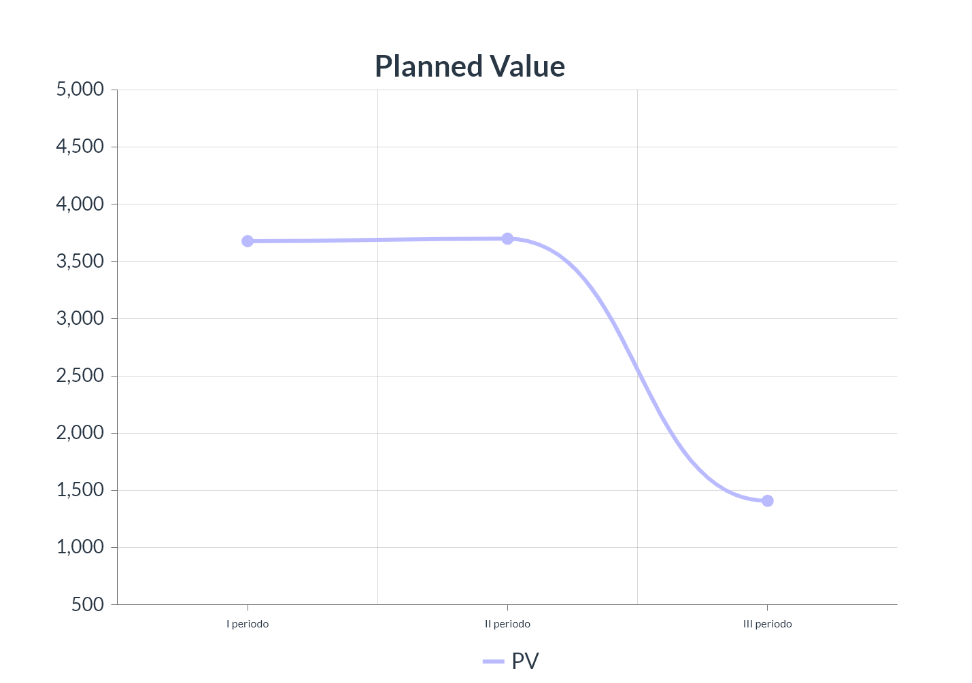
\includegraphics[width=10cm]{./res/images/PVGraph.png}
  \caption{Planned Value}
  \label{fig:Grafico Planned Value}
\end{figure}
\end{center}

\begin{center}
\begin{figure}[H]
  \centering
  \renewcommand{\thefigure}{2}
  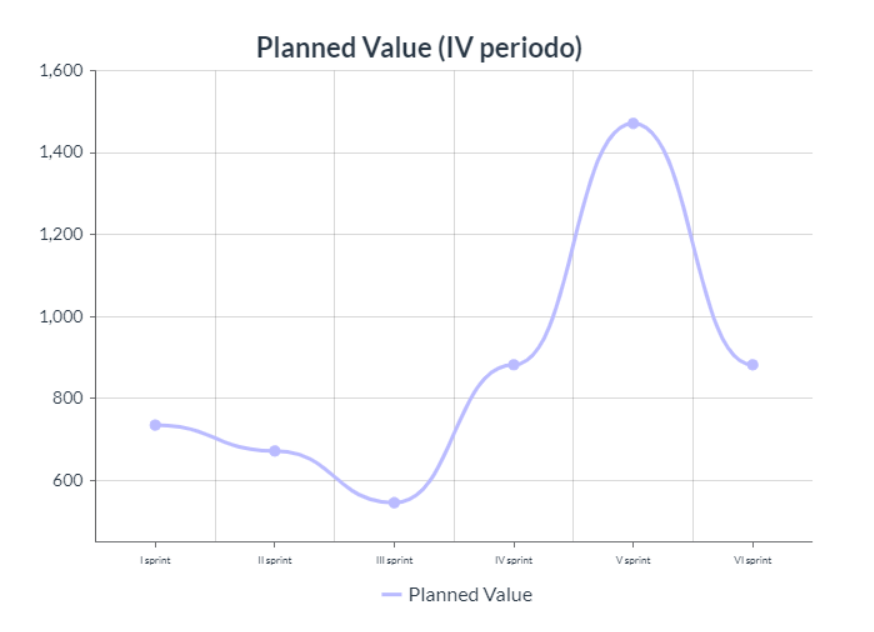
\includegraphics[width=10cm]{./res/images/PVGraphSprint.png}
  \caption{Planned Value (IV periodo)}
  \label{fig:Grafico Planned Value (IV periodo)}
\end{figure}
\end{center}
Nel terzo periodo la differenza è molto bassa date le poche ore lavorative. Queste poche ore pianificate, come sottolineato nel Piano di Progetto, son state dovute a festività, impegni accademici e per la rallentamenti dovuti alla revisione.\\ 
Il quarto e ultimo periodo che raggruppa 5 Sprint è stato quello con più ore pianificate data la mole di lavoro finale da effettuare: completamento dei documenti e aggiornamenti, fase di progettazione dell’architettura, fase di codifica del prodotto, testing. Un maggiore monte ore equivale ad un maggior valore atteso, per questo motivo l’ultimo periodo risale di molto nel grafico.
\\
\paragraph{Actual Cost}
\begin{center}
\begin{figure}[H]
  \centering
  \renewcommand{\thefigure}{3}
  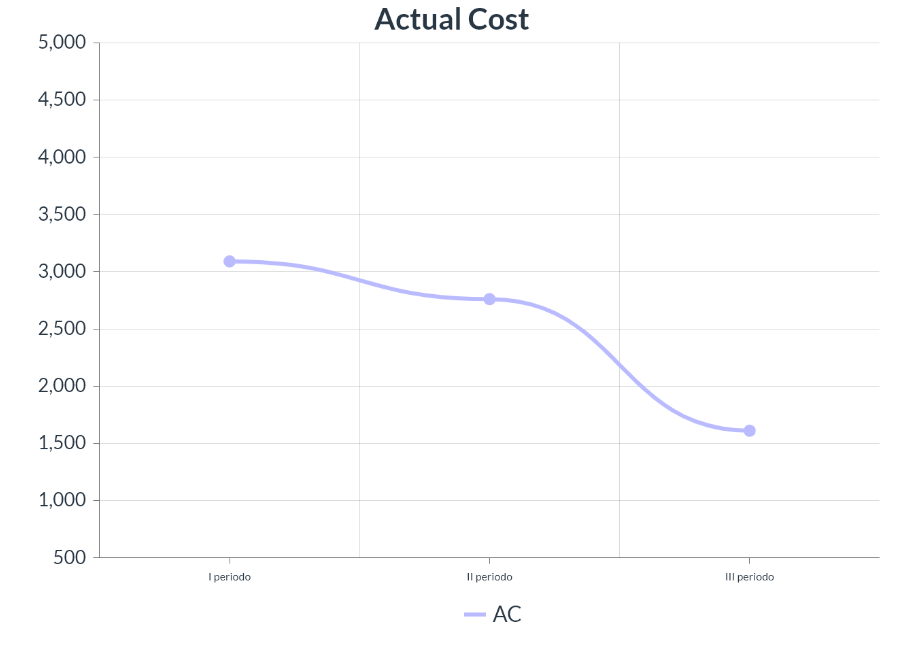
\includegraphics[width=10cm]{./res/images/ACGraph.png}
  \caption{Actual Cost}
  \label{fig:Grafico Actual Cost}
\end{figure}
\end{center}
Dal grafico si può notare come nel terzo periodo la differenza è bassa poichè abbiamo effettuato 90 ore lavorative e quindi prodotto poco valore. Questo periodo è registrato e spiegato nel \textit{Piano di Progetto}.
\begin{center}
\begin{figure}[H]
  \centering
  \renewcommand{\thefigure}{4}
  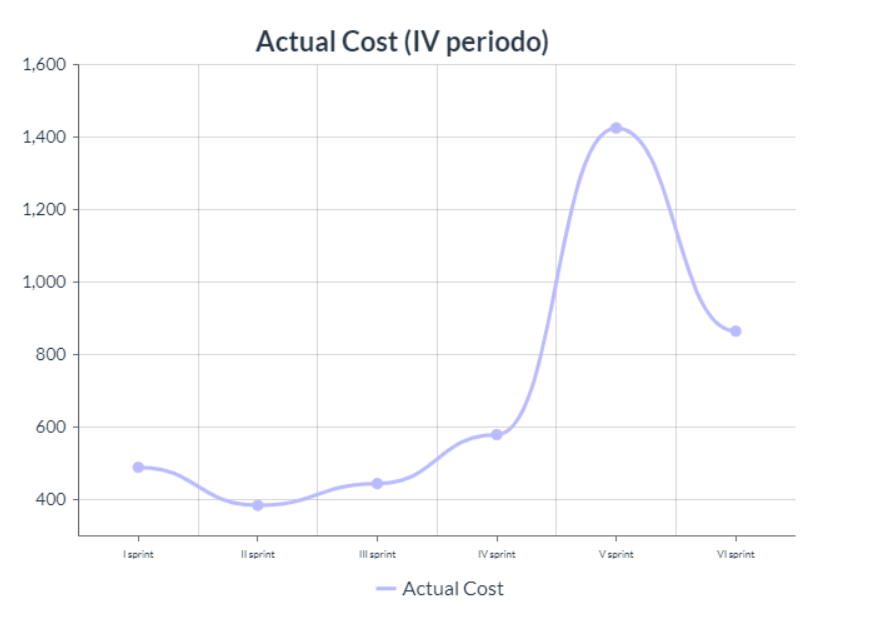
\includegraphics[width=10cm]{./res/images/ACGraphSprint.png}
  \caption{Actual Cost (IV periodo)}
  \label{fig:Grafico Actual Cost (IV periodo)}
\end{figure}
\end{center}
Nel quarto ed ultimo periodo invece l'Actual Cost è salito di molto utilizzando 230 delle 247 ore pianificate, di conseguenza il valore è aumentato notevolmente.\\
Si può notare un picco nel V Sprint date le 70 ore lavorative impiegate.
\paragraph{Earned Value}
\begin{center}
\begin{figure}[H]
  \centering
  \renewcommand{\thefigure}{5}
  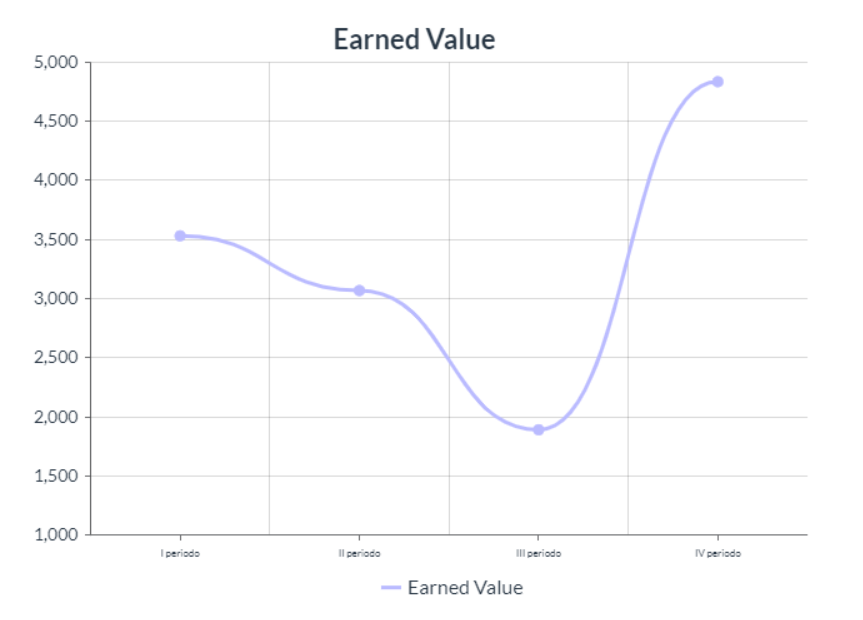
\includegraphics[width=10cm]{./res/images/EVGraph.png}
  \caption{Earned Value}
  \label{fig:Grafico Earned Value}
\end{figure}
\end{center}
Da come si nota dal grafico nei primi tre periodi l'Earned Value è andato a calare in quanto dal primo al secondo c'è stata una lieve diminuzione delle ore impiegate, mentre nel terzo periodo il quantitativo di ore utilizzato è stato dimezzato date le problematiche descritte.
\begin{center}
\begin{figure}[H]
  \centering
  \renewcommand{\thefigure}{6}
  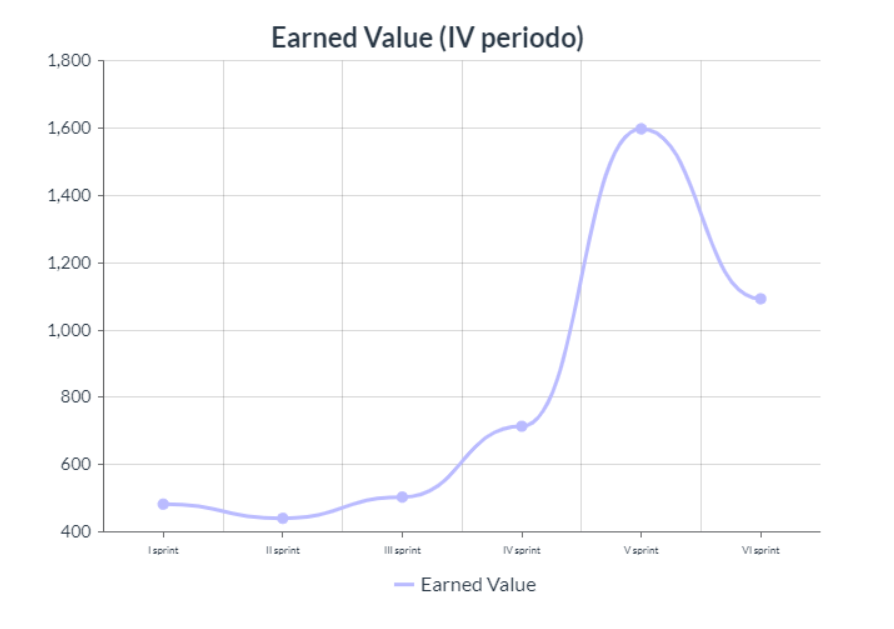
\includegraphics[width=10cm]{./res/images/EVGraphSprint.png}
  \caption{Earned Value (IV periodo)}
  \label{fig:Grafico Earned Value (IV periodo)}
\end{figure}
\end{center}
Il quarto ed ultimo periodo invece ha alzato l'Earned Value dato il carico di lavoro che avevamo da svolgere e le ore che ci abbiamo impiegato.\\
Gli ultimi tre Sprint sono stati decisivi, dato che successivamente ai primi 3, avevamo le idee più chiare e sapevamo come dividerci il lavoro e come agire.
\paragraph{Cost Variance}
\begin{center}
\begin{figure}[H]
  \centering
  \renewcommand{\thefigure}{7}
  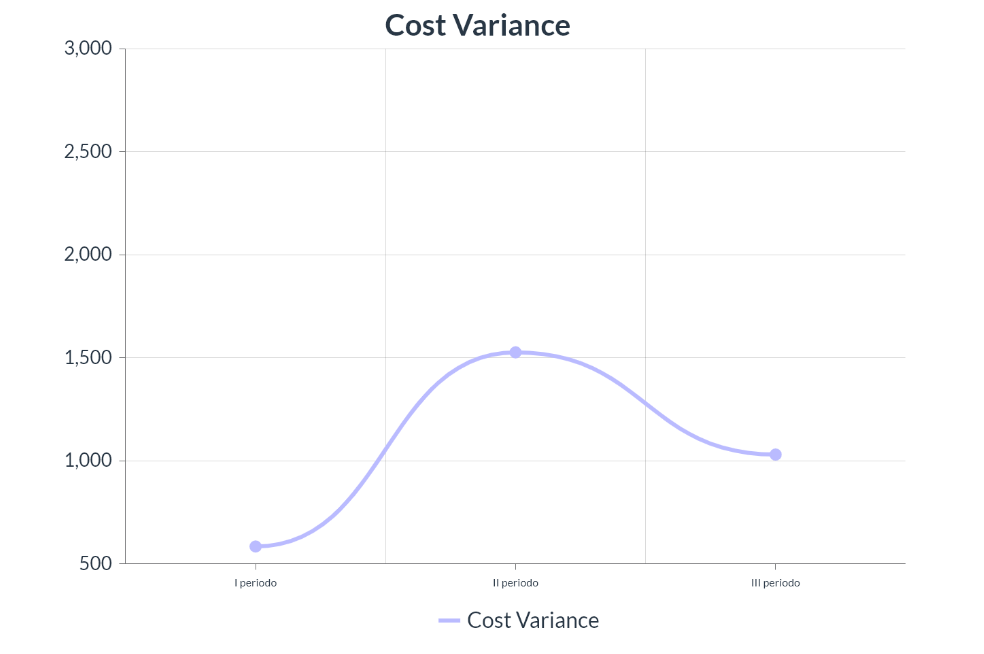
\includegraphics[width=10cm]{./res/images/CVGraph.png}
  \caption{Cost Variance}
  \label{fig:Grafico Cost Variance}
\end{figure}
\end{center}
Il grafico rappresenta le misure in considerazione per calcolare la Cost Variance.\\ 
Più il valore di scarto è alto, più è alta l’efficienza con cui si sta lavorando risparmiando sul costo pianificato. Essendo riusciti sempre a completare il lavoro con ore risparmiate questa misura la si può notare sempre in aumento. In particolare nell’ultimo periodo poichè siamo riusciti a raggiungere la fine del prodotto risparmiando dalle ore pianificate e budget stanziato (come descritto nel documento \textit{Piano di Progetto}).
\begin{center}
\begin{figure}[H]
  \centering
  \renewcommand{\thefigure}{8}
  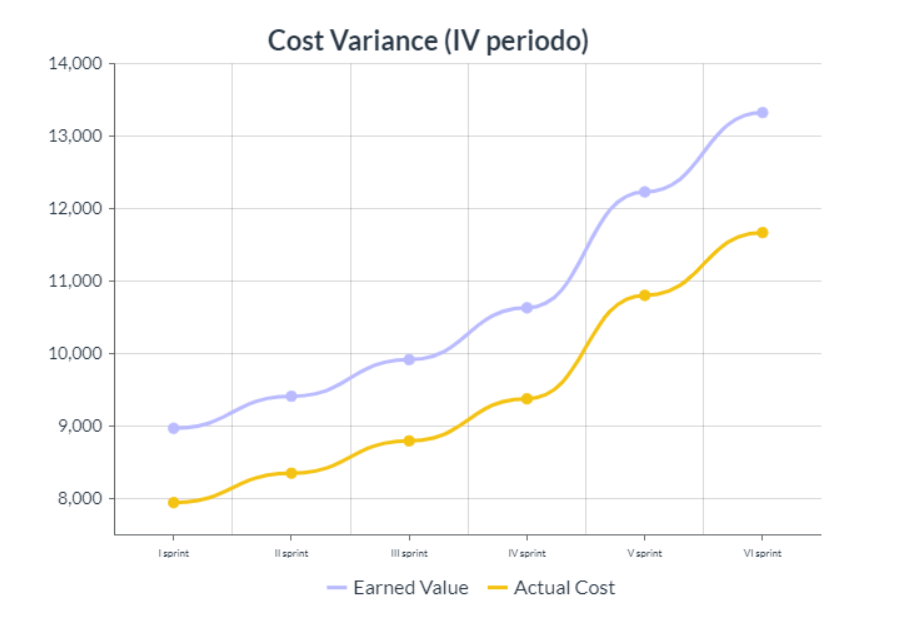
\includegraphics[width=10cm]{./res/images/CVGraphSprint.png}
  \caption{Cost Variance (IV periodo)}
  \label{fig:Grafico Cost Variance (IV periodo)}
\end{figure}
\end{center}

\paragraph{Schedule Variance}
\begin{center}
\begin{figure}[H]
  \centering
  \renewcommand{\thefigure}{9}
  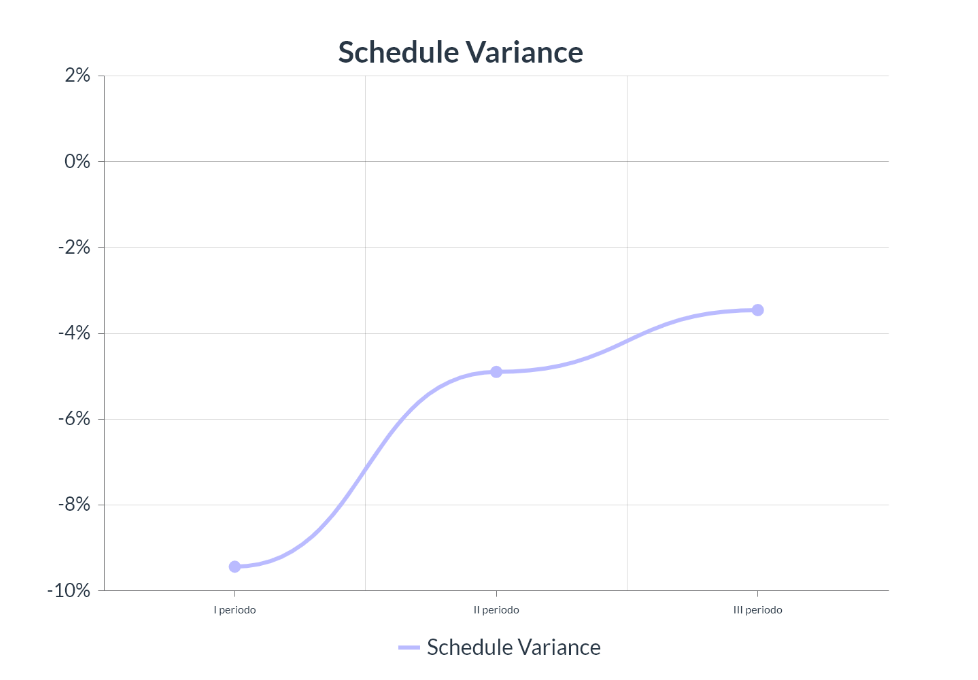
\includegraphics[width=10cm]{./res/images/SVGraph.png}
  \caption{Schedule Variance}
  \label{fig:Grafico Schedule Variance}
\end{figure}
\end{center}
Dal II periodo si nota un sostanziale miglioramento in quanto abbiamo mantenuto un monte ore molto alto come nel I periodo, cosa che non abbiamo fatto nel terzo e per quello non c'è stato un cambiamento significativo. Nel quarto ed ultimo invece la differenza tra il valore aspettato e il valore effettivo è diventato più grande, per questo motivo la percentuale si è alzata, dato che abbiamo utilizzato meno ore per effettuare alcuni sprint e di conseguenza il valore è risultato ridotto.
\begin{center}
\begin{figure}[H]
  \centering
  \renewcommand{\thefigure}{10}
  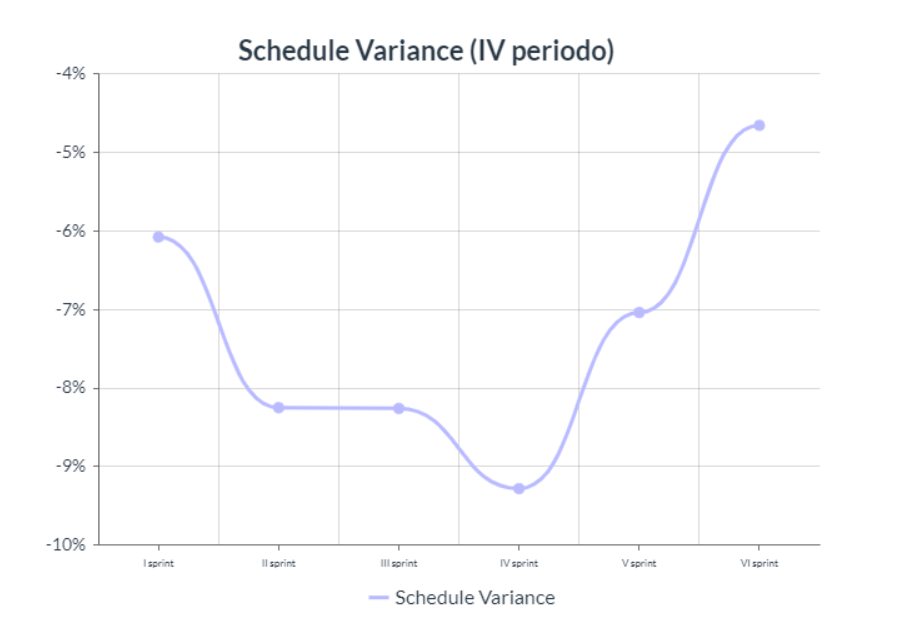
\includegraphics[width=10cm]{./res/images/SVGraphSprint.png}
  \caption{Schedule Variance (IV periodo)}
  \label{fig:Grafico Schedule Variance (IV periodo)}
\end{figure}
\end{center}
Analizzando gli sprint si nota come se avessimo proseguito con lo stesso monte ore utilizzato fino allo sprint 4, la percentuale sarebbe aumentata, invece dopo lo sprint 5, grazie ad un monte ore più alto e all'arrivo della fine del progetto, la percentuale si è abbassata.

\paragraph{Budget Variance}
\begin{center}
\begin{figure}[H]
  \centering
  \renewcommand{\thefigure}{11}
  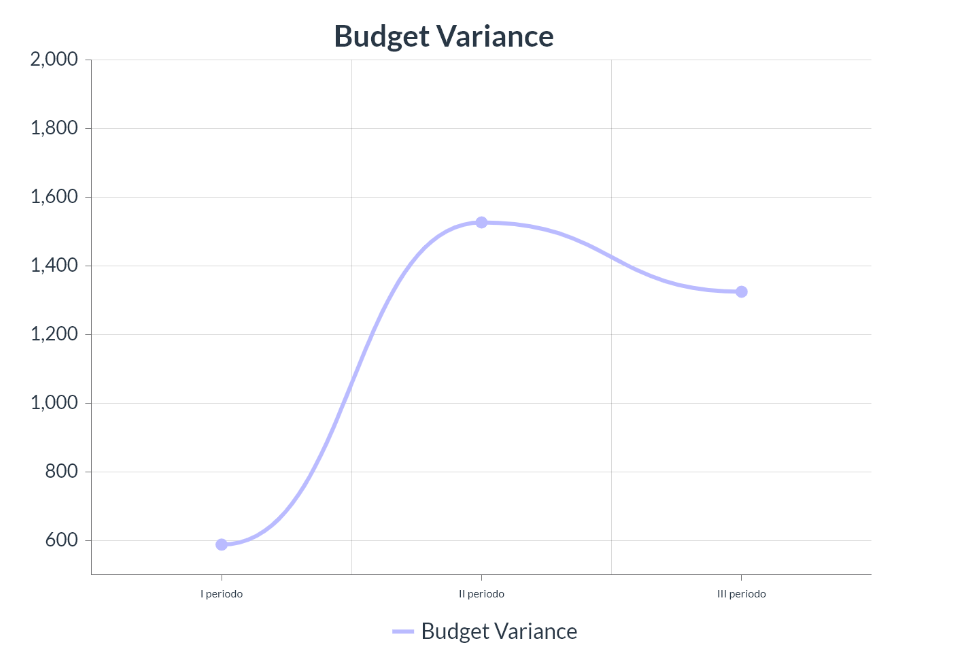
\includegraphics[width=10cm]{./res/images/BVGraph.png}
  \caption{Budget Variance}
  \label{fig:Grafico Budget Variance}
\end{figure}
\end{center}
\begin{center}
\begin{figure}[H]
  \centering
  \renewcommand{\thefigure}{12}
  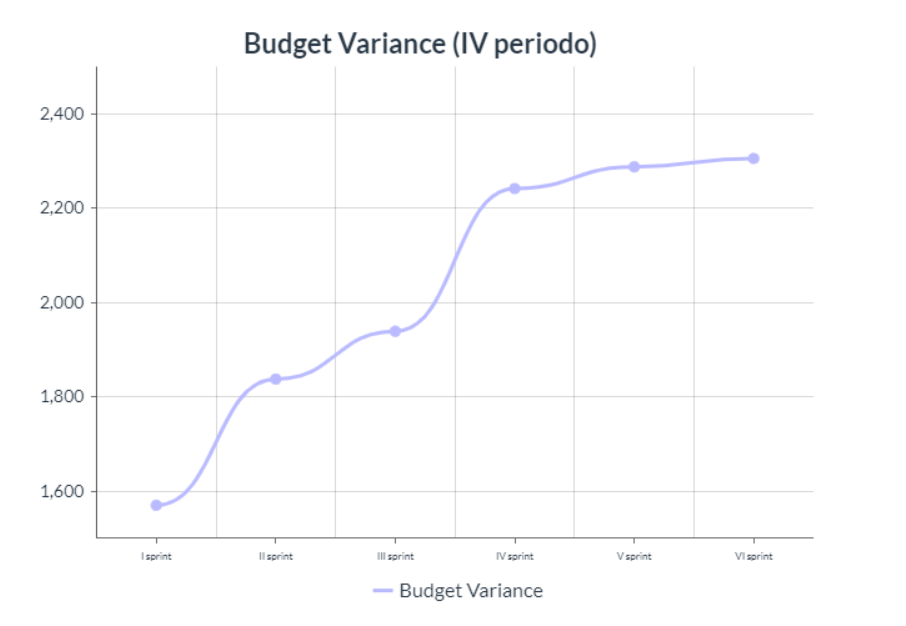
\includegraphics[width=10cm]{./res/images/BVGraphSprint.png}
  \caption{Budget Variance (IV periodo)}
  \label{fig:Grafico Budget Variance (IV periodo)}
\end{figure}
\end{center}
Misura puramente di livello contabile. Se BV \textgreater  0 significa che il progetto sta spendendo il proprio budget con minor velocità di quanto pianificato, viceversa se negativo. Non avendo mai sforato di ore ed avendo terminato il progetto risparmiando ore e budget, il valore è sempre risultato positivo, con un grande incremento nell'ultimo periodo finale.

\subsubsection{Indice di Gulpease}
\noindent Nella seguente tabella vengono riportati gli indici di Gulpease calcolati sulle ultime versioni dei seguenti documenti.\\
Per calcolare i seguenti valori non sono stati considerati: i changelog, la pagina di introduzione del documento, l'indice, tabelle con valori, intestazioni a piè di pagina, captions e la sezione di "Informazioni generali" nei verbali. Sono state incluse invece le colonne di tabelle contenenti descrizioni significative e gli elenchi puntati che contenevano frasi significative. 
\begin{longtable}{ 
		>{\centering}M{0.45\textwidth} 
		>{\centering}M{0.17\textwidth}
		>{\centering}M{0.25\textwidth} 
		}
	\rowcolorhead
	\headertitle{Documento} &
	\centering \headertitle{Valore} &	
	\headertitle{Esito} 
	\endfirsthead	
	\endhead
	
	\textit{Analisi dei Requisiti} & 80 & Superato\tabularnewline
	\textit{Glossario} & 75 & Superato\tabularnewline
	\textit{Norme di Progetto} & 74 & Superato\tabularnewline
	\textit{Piano di Progetto} & 63 & Superato\tabularnewline
	\textit{Piano di Qualifica} & 69 & Superato\tabularnewline
	\textit{Studio di Fattibilità} & 80 & Superato\tabularnewline
	VE 22-10-25 & 82 & Superato\tabularnewline
	VE 22-10-26 & 84 & Superato\tabularnewline
	VE 22-11-17	& 75 & Superato\tabularnewline
	VE 23-01-11	& 57 & Superato\tabularnewline
	VE 23-01-18	& 69 & Superato\tabularnewline
	VE 23-02-17 & 70 & Superato\tabularnewline
	VE 23-04-05 & 60 & Superato\tabularnewline
	VE 23-04-14 & 63 & Superato\tabularnewline
	VE 23-05-12 & 64 & Superato\tabularnewline
	VI 22-10-25 & 74 & Superato\tabularnewline
	VI 22-10-26 & 79 & Superato\tabularnewline
	VI 22-11-04 & 63 & Superato\tabularnewline
	VI 22-11-09 & 88 & Superato\tabularnewline
	VI 22-11-16 & 63 & Superato\tabularnewline
	VI 22-11-23 & 72 & Superato\tabularnewline
	VI 22-12-01 & 60 & Superato\tabularnewline
	VI 22-12-07 & 78 & Superato\tabularnewline
	VI 22-12-14 & 69 & Superato\tabularnewline
	VI 23-01-04 & 63 & Superato\tabularnewline
	VI 23-01-25 & 68 & Superato\tabularnewline
	VI 23-02-01 & 65 & Superato\tabularnewline
	VI 23-02-08 & 58 & Superato\tabularnewline
	VI 23-02-24 & 68 & Superato\tabularnewline
	VI 23-02-28 & 65 & Superato\tabularnewline
	VI 23-03-16 & 67 & Superato\tabularnewline
	VI 23-04-19 & 70 & Superato\tabularnewline
	VI 23-04-23 & 70 & Superato\tabularnewline
	VI 23-05-05 & 67 & Superato\tabularnewline
	VI 23-05-29 & 70 & Superato\tabularnewline
	
\end{longtable}

\begin{center}
\begin{figure}[H]
  \centering
  \renewcommand{\thefigure}{13}
  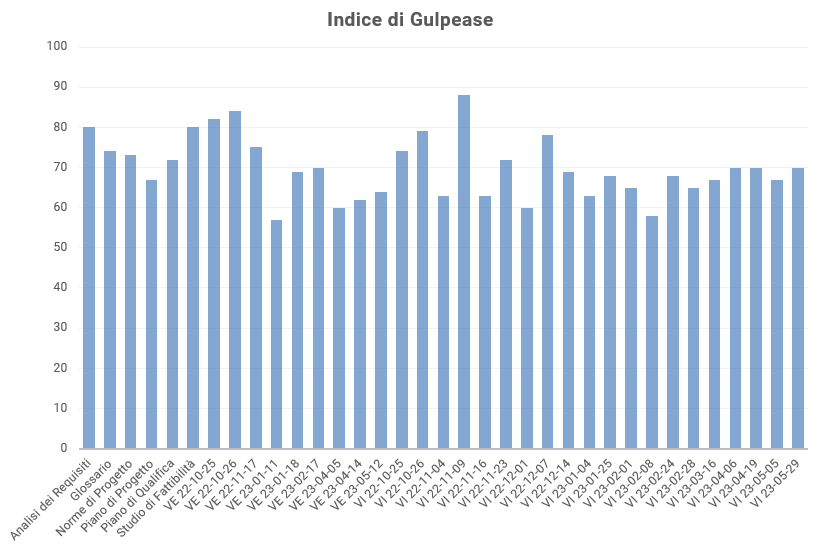
\includegraphics[width=10cm]{./res/images/GulpeaseGen.png}
  \caption{Indice di Gulpease dei documenti}
  \label{fig:Indice di Gulpease dei documenti}
\end{figure}
\end{center}
\noindent Qui ora vengono riportati i grafici che analizzano l'andamento dell'indice di Gulpease di documenti in continua evoluzione.
\paragraph{Indice di Gulpease - \textit{Analisi dei Requisiti}}
\begin{center}
\begin{figure}[H]
  \centering
  \renewcommand{\thefigure}{14}
  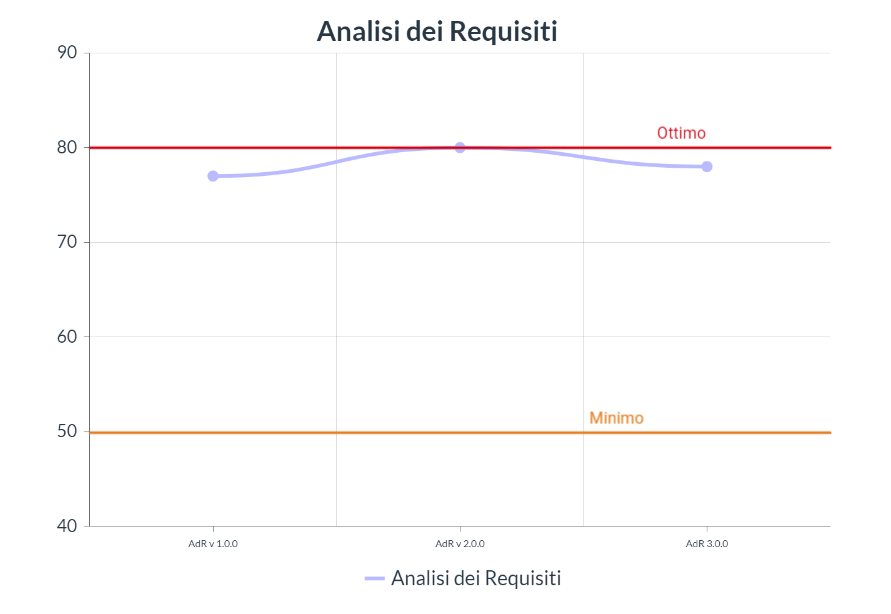
\includegraphics[width=10cm]{./res/images/AdRGraph.png}
  \caption{Indice di Gulpease - \textit{Analisi dei Requisiti}}
  \label{fig:Indice di Gulpease - Analisi dei Requisiti}
\end{figure}
\end{center}
\paragraph{Indice di Gulpease - \textit{Norme di Progetto}}
\begin{center}
\begin{figure}[H]
  \centering
  \renewcommand{\thefigure}{15}
  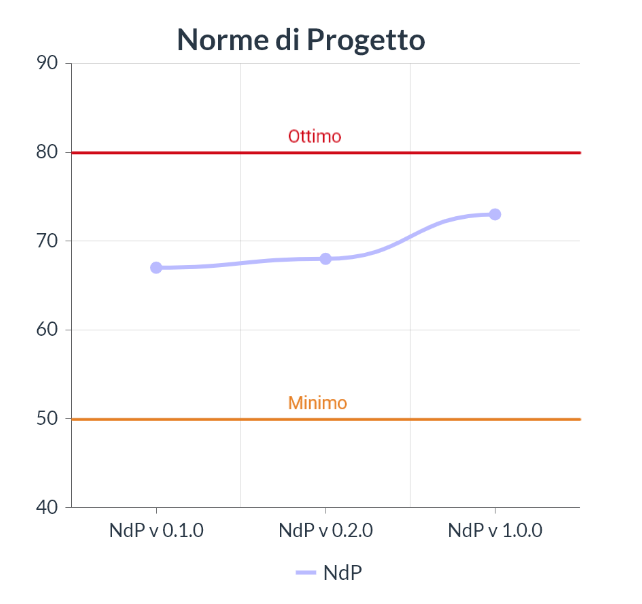
\includegraphics[width=10cm]{./res/images/NdPGraph.png}
  \caption{Indice di Gulpease - \textit{Norme di Progetto}}
  \label{fig:Indice di Gulpease - Norme di Progetto}
\end{figure}
\end{center}
\paragraph{Indice di Gulpease - \textit{Piano di Progetto}}
\begin{center}
\begin{figure}[H]
  \centering
  \renewcommand{\thefigure}{16}
  \includegraphics[width=10cm]{./res/images/PdPGraph.png}
  \caption{Indice di Gulpease - \textit{Piano di Progetto}}
  \label{fig:Indice di Gulpease - Piano di Progetto}
\end{figure}
\end{center}
\paragraph{Indice di Gulpease - \textit{Piano di Qualifica}}
\begin{center}
\begin{figure}[H]
  \centering
  \renewcommand{\thefigure}{17}
  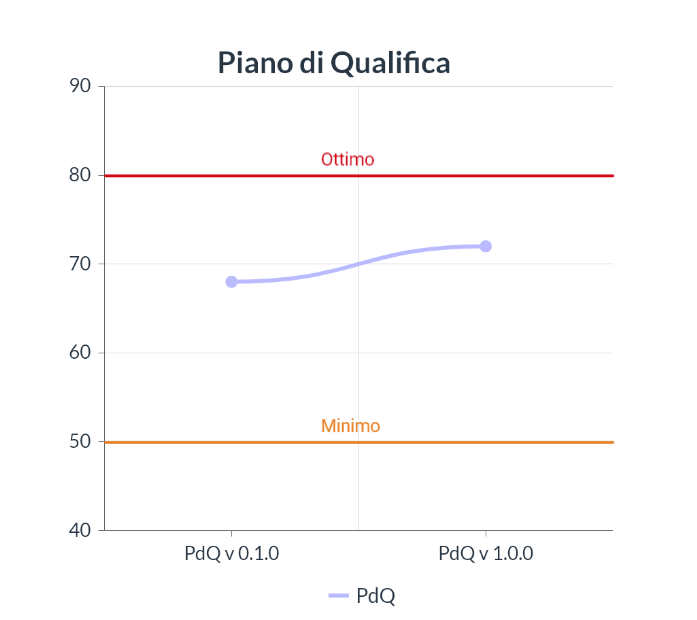
\includegraphics[width=10cm]{./res/images/PdQGraph.png}
  \caption{Indice di Gulpease - \textit{Piano di Qualifica}}
  \label{fig:Indice di Gulpease - Piano di Qualifica}
\end{figure}
\end{center}
\pagebreak
\subsection{Verifica della qualità dei prodotti\textsubscript{g}}
In questa sezione vengono riportati i risultati dell'attività di verifica\textsubscript{g} effettuata relativa alla qualità del prodotto\textsubscript{g}.\\

\begin{longtable}{ 
		>{\centering}M{0.45\textwidth} 
		>{\centering}M{0.17\textwidth}
		>{\centering}M{0.25\textwidth} 
		}
	\rowcolorhead
	\headertitle{Metrica} &
	\centering \headertitle{Valore} &	
	\headertitle{Esito} 
	\endfirsthead	
	\endhead
	Percentuale di requisiti soddisfatti& 100\% Obbligatori + 28\% Facoltativi  & Superato\tabularnewline
	Densità di fallimenti durante l'esecuzione& 15\% & Superato\tabularnewline
	Tempo medio di risposta & minore di 1s & Superato\tabularnewline
	Tempo di caricamento& 30 secondi & Non superato\tabularnewline
	Facilità di apprendimento& 90 secondi & Superato\tabularnewline
	Densità dei commenti & 11,05\% & Superato\tabularnewline
	Browser supportati & 100\% & Superato\tabularnewline
\end{longtable}
\noindent Nella seguente tabella è stata calcolata la Complessità Ciclomatica del prodotto.\\
Sono stati inseriti i metodi che presentavano punti decisionali.
Avendo più metodi su ogni modulo è stato deciso di calcolare la media dei metodi per modulo.
\begin{longtable}{ 
		>{\centering}M{0.40\textwidth} 
		>{\centering}M{0.15\textwidth}
		>{\centering}M{0.20\textwidth}
		}
	\rowcolorhead
	\headertitle{Modulo} &
	\headertitle{Valore} &
	\headertitle{Esito} 	
	\endfirsthead	
	\endhead
	Player.jsx & 6 & Superato\tabularnewline
	Model.jsx & 5 & Superato\tabularnewline
	ProductUI.jsx & 12 & Non superato\tabularnewline
	pointerLock.jsx & 4 & Superato\tabularnewline
	Flashlight.jsx & 3 & Superato\tabularnewline
	Raycaster.jsx & 3 & Superato\tabularnewline
	Decoration.jsx & 1,5 & Superato\tabularnewline
	Cart.jsx & 2 & Superato\tabularnewline
	Map.jsx & 1 & Superato\tabularnewline
	useRaycasterLogic.jsx & 0 & Superato\tabularnewline
	CartItem.jsx & 0 & Superato\tabularnewline
	productSlice.js & 2 & Superato\tabularnewline
	Crosshair.jsx & 2 & Superato\tabularnewline
	Scene.jsx & 0 & Superato\tabularnewline
	ProductInteractionPrompt.jsx & 0 & Superato\tabularnewline
	Lights.jsx & 0 & Superato\tabularnewline
	UI.jsx & 0 & Superato\tabularnewline
	cartSlice.js & 0 & Superato\tabularnewline
	
\end{longtable}

Il prodotto è stato testato sui seguenti browser:
\begin{longtable}{ 
		>{\centering}M{0.45\textwidth} 
		>{\centering}M{0.25\textwidth} 
		}
	\rowcolorhead
	\headertitle{Browser} &
	\headertitle{Esito} 
	\endfirsthead	
	\endhead
	
	Google Chrome (versione $ \ge 110 $) & Supportato\tabularnewline
	Microsoft Edge (versione $ \ge 110 $) & Supportato\tabularnewline
	Mozilla Firefox (versione $ \ge 109 $) & Supportato\tabularnewline
	Safari (versione $ \ge 16 $) & Supportato\tabularnewline
	Opera (versione $ \ge 95 $) & Supportato\tabularnewline

\end{longtable}

\section{Specifica dei Test}
\begin{itemize}
\item Test di unità: vengono stabiliti durante la progettazione e servono per verificare le singole unità software;
\item Test di integrazione: vengono stabiliti durante la progettazione e servono per integrare il funzionamento di più unità;
\item Test di accettazione: vengono effettuati insieme al proponente\textsubscript{g} durante la fase di collaudo;
\item Test di sistema: vengono stabiliti durante l'\textit{Analisi dei Requisiti} e servono per accertare la copertura dei requisiti software definiti nel documento di \textit{Analisi dei Requisiti}.
\end{itemize}
Gli acronimi utilizzati in questo documento per identificare i test sono specificati dettagliatamente nel documento di \textit{Norme di Progetto}.
In questa sezione vengono utilizzate le seguenti sigle per lo stato di ogni test:
\begin{itemize}
\item \textbf{S}: test superato
\item \textbf{N}: test non implementato
\end{itemize}

\subsection{Test di unità}
Per garantire il funzionamento dei singoli componenti che possono lavorare in maniera autonoma senza bisogno di dipendenze abbiamo effettuato questi test. Non abbiamo ritenuto necessario testare componenti o parti di componenti che:
\begin{itemize}
	\item Utilizzavano funzionalità già assodate e documentate;
	\item Componenti che raggruppavano altri componenti.
\end{itemize} 
\begin{longtable}{
		>{\centering}M{0.20\textwidth}
		>{\centering}M{0.35\textwidth}	 
		>{\centering}M{0.20\textwidth} 
		}
	\rowcolorhead
	\headertitle{Test} &
	\centering \headertitle{Descrizione} &	
	\headertitle{Stato} 
	\endfirsthead	
	\endhead
TU1 & Si verifichi che la posizione del player cambi quando utilizza i tasti di movimento & S\tabularnewline
TU2 & Si verifichi che la rotazione del player cambi quando muove la visuale col mouse & S\tabularnewline
TU3 & Si verifichi che avvenga il cambiamento colore ad un oggetto interagibile & S\tabularnewline
TU4 & Si verifichi la funzionalità dell’aggiunta all’array che rappresenta gli oggetti nel carrello e l’incremento del costo totale & S\tabularnewline
TU5 & Si verifichi che la funzionalità di aggiungere un oggetto al carrello funzioni solo con oggetti validi & S\tabularnewline
TU6 & Si verifichi la possibilità di utilizzare i selettori Redux per reperire l’array logico del carrello e il costo totale & S\tabularnewline
TU7 & Si verifichi la funzionalità della rimozione totale dall’array del carrello & S\tabularnewline
TU8 & Si verifichi che la funzionalità di rimozione totale dell’array carrello funzioni anche se il carrello è vuoto & S\tabularnewline
TU9 & Si verifichi la funzionalità di eliminazione singola dal carrello & S\tabularnewline
TU10 & Si verifichi che l’eliminazione singola funziona solo con oggetti realmente presenti nell’array carrello & S\tabularnewline
TU11 & Si verifichi che il raycaster funzioni & S\tabularnewline
TU12 & Si verifichi che funzioni la possibilità di aggiungere quantità di un oggetto selezionato & S\tabularnewline
TU13 & Si verifichi che funzioni la possibilità di diminuire quantità di un oggetto selezionato & S\tabularnewline
\end{longtable}

\subsection{Test di integrazione}
Per assicurare che ogni componente lavori correttamente con gli altri componenti, il gruppo ha deciso di effettuare i seguenti Test di Integrazione.
\begin{longtable}{
		>{\centering}M{0.20\textwidth}
		>{\centering}M{0.35\textwidth}	 
		>{\centering}M{0.20\textwidth} 
		}
	\rowcolorhead
	\headertitle{Test} &
	\centering \headertitle{Descrizione} &	
	\headertitle{Stato} 
	\endfirsthead	
	\endhead
TI1 & Si verifichi che la modifica di cambiamento colore venga apportata ad un oggetto esempio nel file JSON contenente i prodotti interagibili & S\tabularnewline
TI2 & Si verifichi che un elemento nel carrello , se eliminato singolarmente, scompaia dal componente Cart e anche dall’array logico del carrello & S\tabularnewline
TI3 & Si verifichi che il bottone “Remove all” funzioni rimuovendo sia da Cart che da cartSlice tutti gli oggetti & S\tabularnewline
TI4 & Si verifichi che il bottone “Remove all” funzioni anche se il carrello è vuoto & S\tabularnewline
TI5 & Si verifichi che il cambio di colore nella Sidebar venga salvato & S\tabularnewline
TI6 & Si verifichi che il colore ritorni a standard se viene deselezionata una modifica di colore & S\tabularnewline
TI7 & Si verifichi che venga aggiunto un oggetto al carrello dalla sidebar & S\tabularnewline
TI8 & Si verifichi che venga aggiunta la quantità selezionata di un oggetto già presente nel carrello & S\tabularnewline
\end{longtable}
\subsection{Test di accettazione}
Questi test verranno stabiliti durante la fase di Collaudo.

\subsection{Test di sistema}
Per assicurare che vengano rispettati i requisiti concordati nel documento di \textit{Analisi dei Requisiti}, vengono eseguiti i seguenti test di sistema.
\begin{longtable}{
		>{\centering}M{0.20\textwidth}
		>{\centering}M{0.35\textwidth}	 
		>{\centering}M{0.20\textwidth} 
		}
	\rowcolorhead
	\headertitle{Test} &
	\centering \headertitle{Descrizione} &	
	\headertitle{Stato} 
	\endfirsthead	
	\endhead
TSRF1 & Si verifica\textsubscript{g} che l'utente possa aggiungere, l'oggetto con cui sta interagendo, nel carrello & S \tabularnewline
TSRF2 & Si verifica\textsubscript{g} che l'utente possa visualizzare il contenuto del carrello & S \tabularnewline
TSRF2.1 & Si verifica\textsubscript{g} che l'utente possa visualizzare la lista degli oggetti presenti nel carrello & S \tabularnewline
TSRF2.1.1 & Si verifica\textsubscript{g} che l'utente possa interagire con un oggetto nel carrello & S \tabularnewline
TSRF2.1.1.1 & Si verifica\textsubscript{g} che l'utente possa visualizzare la caratteristica del nome di ogni oggetto presente nella lista degli oggetti presenti nel carrello & S \tabularnewline
TSRF2.1.1.2 & Si verifica\textsubscript{g} che l'utente possa visualizzare la caratteristica del costo di ogni oggetto presente nella lista degli oggetti presenti nel carrello & S \tabularnewline
TSRF2.1.1.3 & Si verifica\textsubscript{g} che l'utente possa visualizzare la caratteristica della quantità di ogni oggetto presente nella lista degli oggetti presenti nel carrello & S \tabularnewline
TSRF2.2 & Si verifica\textsubscript{g} che l'utente possa visualizzare il costo totale degli oggetti che ha inserito nel carrello & S \tabularnewline
TSRF3 & Si verifica\textsubscript{g} che l'utente abbia la possibilità di rimuovere tutti gli oggetti dal carrello & S \tabularnewline
TSRF4 & Si verifica\textsubscript{g} che l'utente abbia la possibilità di rimuovere un singolo oggetto dal carrello & S \tabularnewline
TSRF5 & Si verifica\textsubscript{g} che l'utente possa muoversi in maniera direzionale & S \tabularnewline
TSRF5.1 & Si verifica\textsubscript{g} che l'utente possa compiere movimenti direzionali nell'asse X & S \tabularnewline
TSRF5.2 & Si verifica\textsubscript{g} che l'utente possa compiere movimenti direzionali nell'asse Y & S \tabularnewline
TSRF5.3 & Si verifica\textsubscript{g} che l'utente possa compiere movimenti direzionali nell'asse Z & S \tabularnewline
TSRF6 & Si verifica\textsubscript{g} che l'utente possa compiere spostamenti di camera & S \tabularnewline
TSRF6.1 & Si verifica\textsubscript{g} che l'utente possa compiere spostamenti di camera nell'asse X & S \tabularnewline
TSRF6.2 & Si verifica\textsubscript{g} che l'utente possa compiere spostamenti di camera nell'asse Y & S \tabularnewline
TSRF7 & Si verifica\textsubscript{g} che l'utente possa modificare la combinazione dei colori di un oggetto & S \tabularnewline
TSRF8 & Si verifica\textsubscript{g} che l'utente venga notificato in caso non fosse possibile modificare un oggetto & S \tabularnewline
TSRF9 & Si verifica\textsubscript{g} che l'utente possa visualizzare la lista degli oggetti della stanza in cui si trova & N \tabularnewline
TSRF9.1 & Si verifica\textsubscript{g} che l'utente possa visualizzare un singolo oggetto nella lista degli oggetti della stanza in cui si trova & N \tabularnewline
TSRF9.1.1 & Si verifica\textsubscript{g} che l'utente possa visualizzare la caratteristica del nome di ogni oggetto della lista degli oggetti della stanza in cui si trova & N \tabularnewline
TSRF10 & Si verifica\textsubscript{g} che l'utente possa visualizzare tutti i dettagli di un oggetto selezionato & S \tabularnewline
TSRF11 & Si verifica\textsubscript{g} che l'utente abbia la possibilità di riposizionarsi vicino ad un oggetto nella stanza in cui si trova & N \tabularnewline
TSRF12 & Si verifica\textsubscript{g} che l'utente possa riposizionarsi in una stanza da lui selezionata & N \tabularnewline
TSRF13 & Si verifica\textsubscript{g} che l'utente venga notificato in caso il riposizionamento in una stanza non sia possibile & N \tabularnewline
TSRF14 & Si verifica\textsubscript{g} che l'utente venga notificato in caso il riposizionamento in prossimità di un oggetto selezionato non sia concesso & N \tabularnewline
TSRF15 & Si verifica\textsubscript{g} che l'utente possa visualizzare la lista delle stanze & N \tabularnewline
TSRF15.1 & Si verifica\textsubscript{g} che l'utente possa visualizzare una singola stanza dalla lista delle stanze & N \tabularnewline
TSRF15.1.1 & Si verifica\textsubscript{g} che l'utente possa visualizzare la caratteristica del nome di ogni stanza dalla lista delle stanze & N \tabularnewline
TSRF15.1.2 & Si verifica\textsubscript{g} che l'utente possa visualizzare la caratteristica della tipologia di oggetti presenti in ogni stanza nella lista delle stanze & N \tabularnewline
TSRF16 & Si verifica\textsubscript{g} che l'utente possa riposizionare un oggetto presente nella stanza in cui si trova & N \tabularnewline
TSRF17 & Si verifica\textsubscript{g} che l'utente non possa riposizionare un oggetto in una coordinata non legittima & N \tabularnewline
TSRF18 & Si verifica\textsubscript{g} che l'utente sia in grado ad illuminare l'ambiente davanti a lui & S \tabularnewline
TSRF19 & Si verifica\textsubscript{g} che l'utente venga notificato se il contenuto del carrello è vuoto & S \tabularnewline
TSRF20 & Si verifica\textsubscript{g} che l'utente possa visualizzare un oggetto illuminato & S \tabularnewline
\end{longtable}

\subsection{Tracciamento dei test}
\subsubsection{Test di Sistema - Requisiti}
\begin{longtable}{
		>{\centering}M{0.25\textwidth}
		>{\centering}M{0.25\textwidth}	 
		}
	\rowcolorhead
	\headertitle{Test di sistema} &
	\headertitle{Requisiti}
	\endfirsthead	
	\endhead
TSRF1 & RF1\tabularnewline
TSRF2 & RF2\tabularnewline
TSRF2.1 & RF2.1\tabularnewline
TSRF2.1.1 & RF2.1.1\tabularnewline
TSRF2.1.1.1 & RF2.1.1.1\tabularnewline
TSRF2.1.1.2 & RF2.1.1.2\tabularnewline
TSRF2.1.1.3 & RF2.1.1.3\tabularnewline
TSRF2.2 & RF2.2\tabularnewline
TSRF3 & RF3\tabularnewline
TSRF4 & RF4\tabularnewline
TSRF5 & RF5\tabularnewline
TSRF5.1 & RF5.1\tabularnewline
TSRF5.2 & RF5.2\tabularnewline
TSRF5.3 & RF5.3\tabularnewline
TSRF6 & RF6\tabularnewline
TSRF7 & RF7\tabularnewline
TSRF8 & RF8\tabularnewline
TSRF9 & RF9\tabularnewline
TSRF9.1 & RF9.1\tabularnewline
TSRF9.1.1 & RF9.1.1\tabularnewline
TSRF10 & RF10\tabularnewline
TSRF11 & RF11\tabularnewline
TSRF12 & RF12\tabularnewline
TSRF13 & RF13\tabularnewline
TSRF14 & RF14\tabularnewline
TSRF15 & RF15\tabularnewline
TSRF15.1 & RF5.1\tabularnewline
TSRF15.1.1 & RF15.1.1\tabularnewline
TSRF15.1.2 & RF15.1.2\tabularnewline
TSRF16 & RF16\tabularnewline
TSRF17 & RF17\tabularnewline
TSRF18 & RF18\tabularnewline
TSRF19 & RF19\tabularnewline
TSRF20 & RF20\tabularnewline

\end{longtable}

\subsubsection{Test di Unità - File di Test}
\begin{longtable}{
		>{\centering}M{0.10\textwidth}
		>{\centering}M{0.30\textwidth}
		>{\centering}M{0.45\textwidth}	 
		}
	\rowcolorhead
	\headertitle{Test} &
	\centering \headertitle{File di test} &	
	\centering \headertitle{Nome test} 
	\endfirsthead	
	\endhead
TU1 & \_\_test\_\_/playerSlice.test.js & it(’should set the player position’)\{ … \}\tabularnewline
TU2 & \_\_test\_\_/playerSlice.test.js & it(’should set the player rotation’)\{ … \}\tabularnewline
TU3 & \_\_test\_\_/productSlice.test.js & it('Should change color to the product in example')\{ … \}\tabularnewline
TU4 & \_\_test\_\_/cartSlice.test.js & it('Should add an item to the array (that represents the logic of the cart) of the slice and increment the totalCost’)\{ … \}\tabularnewline
TU5 & \_\_test\_\_/cartSlice.test.js & it('Should not be able to add this item’) \{ … \}\tabularnewline
TU6 & \_\_test\_\_/cartSlice.test.js & it('Should be able to use the cartItems selector and the totalCost selector’)\{ … \}\tabularnewline
TU7 & \_\_test\_\_/cartSlice.test.js & it('Should remove all the item in the cart')\{ … \}\tabularnewline
TU8 & \_\_test\_\_/cartSlice.test.js & it('Should remove all the items even if the cart is empty’)\{ … \}\tabularnewline
TU9 & \_\_test\_\_/cartSlice.test.js & it('Should remove the item in example’)\{ … \}\tabularnewline
TU10 & \_\_test\_\_/cartSlice.test.js & it('Should be able to work even if the item provided do not exist in the cart’)\{ … \}\tabularnewline
TU11 & \_\_test\_\_/useRaycasterLogic.test.js & it('should update intersects when mouse moves’)\{ … \}\tabularnewline
TU12 & \_\_test\_\_/productSidebar.test.js & it('Should add more then one quantity of the item selected’)\{ … \}\tabularnewline
TU13 & \_\_test\_\_/productSidebar.test.js & it('Should decrease of one the quantity of the item’)\{ … \}\tabularnewline
\end{longtable}

\subsubsection{Test di Integrità - File di Test}
\begin{longtable}{
		>{\centering}M{0.10\textwidth}
		>{\centering}M{0.30\textwidth}
		>{\centering}M{0.45\textwidth}	 
		}
	\rowcolorhead
	\headertitle{Test} &
	\centering \headertitle{File di test} &	
	\centering \headertitle{Nome test} 
	\endfirsthead	
	\endhead
TI1 & \_\_test\_\_/productSlice.test.js & it('Should change color to the product with the ID=1 imported from the JSON file’)\{ … \} \tabularnewline
TI2 & \_\_test\_\_/cart.test.js & it('Should stop rendering item in cart when clicking "X" button’)\{ … \}\tabularnewline
TI3 & \_\_test\_\_/cart.test.js & it('Should stop rendering all items in cart when clicking "Remove all" button’)\{ … \}\tabularnewline
TI4 & \_\_test\_\_/cart.test.js & it('Should try to remove the items and work even if cart is empty’)\{ … \}\tabularnewline
TI5	& \_\_test\_\_/productSidebar.test.js & it('Should change the variable selectedColor to the product in example’)\{ … \}\tabularnewline
TI6 & \_\_test\_\_/productSidebar.test.js & it('Should remove the selected color if the button with the current color is pressed, putting the standard color to the item’)\{ … \}\tabularnewline
TI7 & \_\_test\_\_/productSidebar.test.js & it('Should add an item to the cart’)\{ … \}\tabularnewline
TI8 & \_\_test\_\_/productSidebar.test.js & it('Should add more than one quantity of the item to the cart, testing also if it adds the quantity to the item that is already in the cart’)\{ … \}\tabularnewline
\end{longtable}